\documentclass[11pt,a4paper]{article}
\usepackage[utf8]{inputenc}
\usepackage[T1]{fontenc}
\usepackage{geometry}
\geometry{margin=1in}
\usepackage{graphicx}
\usepackage{hyperref}
\usepackage{listings}
\usepackage{xcolor}
\usepackage{float}
\usepackage{caption}
\usepackage{subcaption}
\usepackage{amsmath}
\usepackage{amssymb}
\usepackage{booktabs}
\usepackage{array}
\usepackage{multirow}
\usepackage{enumitem}
\usepackage{fancyhdr}
\usepackage{titlesec}
\usepackage{parskip}
\usepackage{setspace}
\usepackage{abstract}
\usepackage{tikz}
\usetikzlibrary{shapes, arrows, positioning, shadows}

% Set up hyperref
\hypersetup{
	colorlinks=true,
	linkcolor=blue,
	urlcolor=blue,
	citecolor=blue
}

% Code listing style
\lstset{
	language=Fortran,
	basicstyle=\ttfamily\small,
	keywordstyle=\color{blue}\bfseries,
	commentstyle=\color{green!60!black},
	stringstyle=\color{red},
	numbers=left,
	numberstyle=\tiny\color{gray},
	frame=single,
	breaklines=true,
	captionpos=b,
	tabsize=4,
	showspaces=false,
	showstringspaces=false
}

% Page style
\pagestyle{fancy}
\fancyhf{}
\fancyhead[L]{\leftmark}
\fancyhead[R]{Compiler-Driven Parallelism in Modern Fortran}
\fancyfoot[C]{\thepage}

% Title formatting
\titleformat{\section}{\Large\bfseries}{\thesection}{1em}{}
\titleformat{\subsection}{\large\bfseries}{\thesubsection}{1em}{}

\begin{document}
	
	% ==================== PAGE 1 — TITLE PAGE ====================
	\begin{titlepage}
		\centering
		\vspace*{1cm}
		
		\Huge
		\textbf{Compiler-Driven Parallelism in Modern Fortran}\\[0.5cm]
		\textbf{using DO CONCURRENT}
		
		\vspace{0.5cm}
		\Large
		Technical Report
		
		\vspace{2cm}
		
		\normalsize

		
		\begin{tabular}{rl}
			\textbf{Author:} & Shahid Maqbool \\
			\textbf{Version:} & 1.0.0 \\
			\textbf{Date:} & \today \\
			\textbf{GitHub Repository:} & \parbox{0.5\textwidth}{\href{https://github.com}{://https://github.com/Shahid718/Compiler-Driven-Parallelism-in-Modern-Fortran-using-DO-CONCURRENT}} \\
			\textbf{License:} & MIT License
		\end{tabular}
		
		% ====================  — ABSTRACT ====================
		\vspace{3cm}
		
		\rule{0.8\textwidth}{0.4pt}
		
		\vspace{0.5cm}
		\begin{abstract}
			\noindent
			This document describes the compiler-driven parallelism using the Fortran 2008 \texttt{DO CONCURRENT} construct in a modern Fortran Cahn-Hilliard solver. The report summarizes compiler configuration, benchmarking methodology, and performance analysis on Intel oneAPI and NVIDIA HPC SDK compilers. The primary objective is to demonstrate portable, performance-portable parallelism through standard language constructs, avoiding vendor-specific extensions or external libraries.
		\end{abstract}
		\rule{0.8\textwidth}{0.4pt}
		
		\vfill
	\end{titlepage}
	

	% ==================== Part 3 — INTRODUCTION ====================
	\clearpage
	\section{Introduction}
	\label{sec:introduction}
	
	\subsection{Objectives}
	
	The objective of this repository is to investigate \textbf{portable compiler-driven parallelism} in Modern Fortran using only standard language constructs. Specifically, this work focuses on the \texttt{DO CONCURRENT} construct introduced in Fortran 2008 and significantly enhanced in Fortran 2018.
	
	This repository presents a case study of a Cahn–Hilliard phase-field solver, designed to explore how compilers can leverage \texttt{DO CONCURRENT} to generate parallel code across different hardware architectures without modifying the source code.
	
	\subsection{Motivation}
	
	The HPC landscape is increasingly heterogeneous, with CPUs, GPUs, and accelerators coexisting in modern supercomputing environments. Achieving performance portability—where a single codebase performs well across diverse architectures—remains a significant challenge. Traditional approaches often rely on vendor-specific extensions (e.g., OpenMP, CUDA, OpenACC) or require code duplication for different backends.
	
	\texttt{DO CONCURRENT} offers an alternative: a standard language construct that expresses loop-level parallelism, allowing the compiler to decide to parallelize the code. This approach promises:
	
	\begin{itemize}
		\item \textbf{Why DO CONCURRENT}: A Fortran-standard way to express data-parallel loops without relying on compiler directives or external libraries. DO CONCURRENT automatically enables the compiler to analyze and parallelize loops.
		
		\item \textbf{Why compiler parallelization}: Delegating parallelism decisions to the compiler reduces development overhead and ensures that optimizations remain consistent across platforms as compiler technologies evolve.
		
		\item \textbf{Why portability}: A single source code, compiled with different compilers, can target different architectures—from multi-core CPUs to GPUs—without modifications.
		
		\item \textbf{Why performance portability}: By abstracting the parallelization strategy, \texttt{DO CONCURRENT} allows the compiler to apply architecture-specific optimizations (e.g., vectorization, auto-parallelization, GPU offloading) transparently.
	\end{itemize}
	
	\subsection{Contributions}
	
	This work makes the following contributions:
	
	\begin{itemize}
		\item \textbf{Modern Fortran 2008 implementation}: A clean, modular, and maintainable implementation of the Cahn–Hilliard equation using object-oriented Fortran features.
		
		\item \textbf{Portable parallelism}: Leveraging \texttt{DO CONCURRENT} for portable parallelism across CPU and GPU architectures without compiler directives.
		
		\item \textbf{CMake build system}: A robust build system that simplifies compilation across different platforms and compilers.
		
		\item \textbf{Single and double precision support}: Configurable precision to demonstrate numerical accuracy and performance trade-offs.
		
		\item \textbf{Intel ifx benchmarks}: Comprehensive performance measurements using the Intel oneAPI Fortran compiler.
		
		\item \textbf{NVIDIA nvfortran benchmarks}: Performance analysis using the NVIDIA HPC SDK Fortran compiler.
		
		\item \textbf{Performance analysis}: Detailed analysis of strong scaling, and compiler-specific optimizations.
	\end{itemize}
	
	\subsection{Report Structure}
	
	The remainder of this report is organized as follows: Section~\ref{sec:math} presents the mathematical model of the Cahn–Hilliard equation. Section~\ref{sec:architecture} describes the software architecture and implementation details. Section~\ref{sec:methodology} outlines the benchmarking methodology and compiler configurations. Section~\ref{sec:results} presents the performance results and analysis. Finally, Section~\ref{sec:conclusion} concludes the report and discusses future work.
	
	\section{Mathematical Model}
	\label{sec:math}
	
	The Cahn–Hilliard equation models phase separation and is a fourth-order nonlinear partial differential equation (PDE). In its dimensionless form, it is given by:
	
	\begin{equation}
		\frac{\partial \phi}{\partial t} = M \nabla^2 \left( \frac{\partial f}{\partial \phi} - \kappa^2 \nabla^2 \phi \right)
		\label{eq:ch}
	\end{equation}
	
	where:
	\begin{itemize}
		\item \(\phi\) is the conserved order parameter (concentration field),
		\item \(M\) is the mobility,
		\item \(f(\phi)\) is the homogeneous free energy density,
		\item \(\kappa\) is the gradient energy coefficient,
		\item \(\nabla^2\) is the Laplacian operator.
	\end{itemize}
	
	\section{Numerical Implementation}
	
	The Cahn–Hilliard equation is discretized using finite differences on a uniform grid. An explicit Euler time-stepping scheme is used for temporal discretization, with central differences for spatial derivatives.
	
	For a 2D domain with grid spacing \(\Delta x\) and \(\Delta y\), the Laplacian operator is approximated as:
	
	\begin{equation}
		\nabla^2 \phi_{i,j} \approx \frac{\phi_{i+1,j} - 2\phi_{i,j} + \phi_{i-1,j}}{\Delta x^2} + \frac{\phi_{i,j+1} - 2\phi_{i,j} + \phi_{i,j-1}}{\Delta y^2}
		\label{eq:laplacian}
	\end{equation}
	
	The fourth-order term \(\nabla^4 \phi\) is computed by applying the Laplacian twice:
	
	\begin{equation}
		\nabla^4 \phi_{i,j} = \nabla^2 \left( \nabla^2 \phi_{i,j} \right)
		\label{eq:nabla4}
	\end{equation}
	
	Using explicit Euler time-stepping:
	
	\begin{equation}
		\phi^{n+1}_{i,j} = \phi^{n}_{i,j} + \Delta t M \nabla^2 \left( \frac{\partial f}{\partial \phi} - \kappa^2 \nabla^2 \phi^n_{i,j}  \right)
		\label{eq:euler}
	\end{equation}
	
	where \(\Delta t\) is the time step size.
	
	Periodic boundary conditions are applied on all boundaries, commonly used in phase-field simulations to mimic bulk behavior. For a domain of size \(N_x \times N_y\), the boundary conditions are:
	
	\begin{align}
		\phi_{0,j} &= \phi_{N_x,j} \quad \forall j \in [0, N_y-1] \\
		\phi_{N_x+1,j} &= \phi_{1,j} \quad \forall j \in [0, N_y-1] \\
		\phi_{i,0} &= \phi_{i,N_y} \quad \forall i \in [0, N_x-1] \\
		\phi_{i,N_y+1} &= \phi_{i,1} \quad \forall i \in [0, N_x-1]
	\end{align}
	
	
	% Define block styles
	\tikzset{
		block/.style = {rectangle, draw, fill=blue!10, text width=5.5cm, text centered, 
			minimum height=1.5cm, rounded corners, drop shadow, font=\small},
		arrow/.style = {thick, ->, >=stealth}
	}
	
	\begin{figure}[H]
		\centering
		\begin{tikzpicture}[node distance=1cm, auto]
			
			% Nodes
			\node [block] (init) {Initialization};
			\node [block, below of=init] (chem) {Chemical potential calculation};
			\node [block, below of=chem] (bc) {Boundary conditions application};
			\node [block, below of=bc] (laplacian) {Laplacian computation};
			\node [block, below of=laplacian] (time) {Time integration};
			\node [block, below of=time] (output) {Output};
			
			% Downward arrows between blocks
			\draw [arrow] (chem) -- (init) ;
			\draw [arrow] (bc) -- (chem) ;
			\draw [arrow] (laplacian) -- (bc) ;
			\draw [arrow] (time) -- (laplacian) ;
			\draw [arrow] (output) -- (time) ;
			
			% Iteration loop: from Output back to Initialization
			\draw [arrow, dashed, red!70] (time.west) -- ++(-2.5,0) |- (chem.west)
			node [midway, left, text width=2.8cm, font=\small] {Repeat for the next timestep};
			
		\end{tikzpicture}
		\caption{Numerical implementation flowchart for the Cahn-Hilliard solver.}
		\label{fig:flowchart}
	\end{figure}
	
	\section{Software Architecture}
	\label{sec:architecture}
	The solver adopts a modular design in which computational kernels are separated from supporting infrastructure. The computational kernel modules implement the numerical operations and contain all DO CONCURRENT parallel regions, while the infrastructure modules manage precision, grid initialization, timing, I/O, error handling, and performance reporting etc. This organization improves readability, maintainability, and facilitates future optimization of the performance-critical kernels.	
	Figure~\ref{fig:software_architecture} illustrates the overall software architecture.
	
\begin{figure}[ht]
	\centering
	
	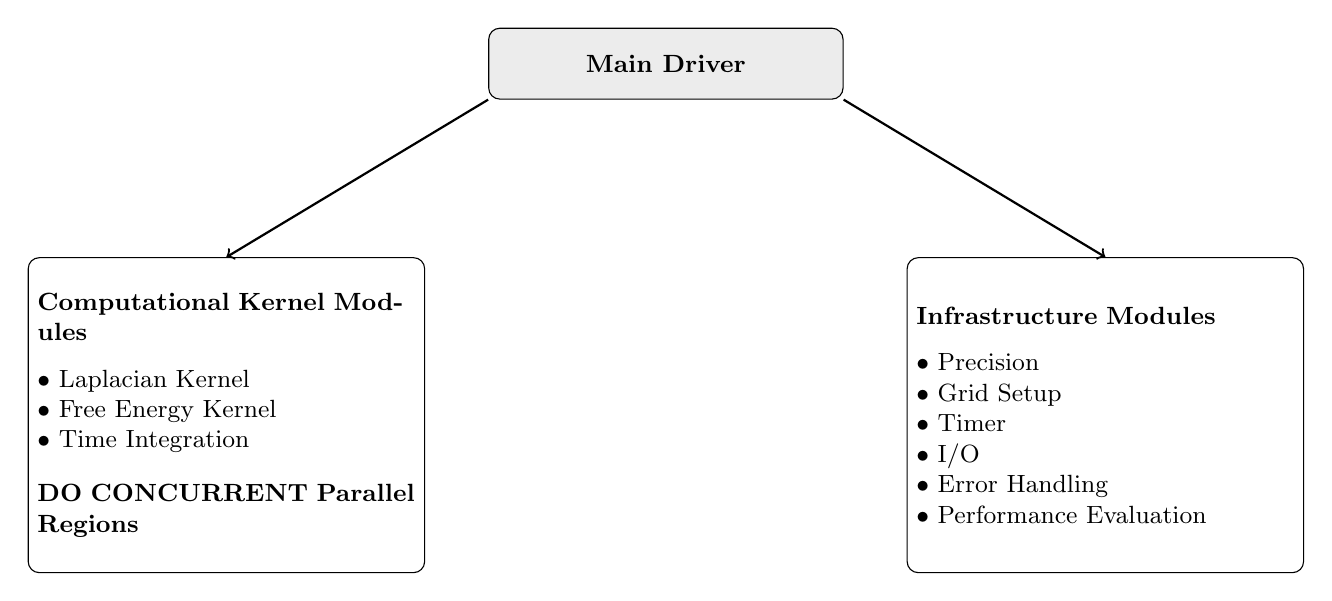
\begin{tikzpicture}[
		node distance=1.8cm,
		every node/.style={font=\small},
		main/.style={
			draw,
			rounded corners,
			fill=gray!15,
			minimum width=4.5cm,
			minimum height=0.9cm,
			align=center
		},
		box/.style={
			draw,
			rounded corners,
			text width=4.8cm,
			align=left,
			minimum height=4.0cm
		}
		]
		
		%--------------------------------------------------
		% Main driver
		%--------------------------------------------------
		\node[main] (main) {\textbf{Main Driver}};
		
		%--------------------------------------------------
		% Left box
		%--------------------------------------------------
		\node[box, below left=2cm and 0.8cm of main] (kernel)
		{
			\textbf{Computational Kernel Modules}
			
			\vspace{0.2cm}
			
			$\bullet$ Laplacian Kernel
			
			$\bullet$ Free Energy Kernel
			
			$\bullet$ Time Integration
			
			\vspace{0.3cm}
			
			\centering
			\textbf{DO CONCURRENT Parallel Regions}
		};
		
		%--------------------------------------------------
		% Right box
		%--------------------------------------------------
		\node[box, below right=2cm and 0.8cm of main] (infra)
		{
			\textbf{Infrastructure Modules}
			
			\vspace{0.2cm}
			
			$\bullet$ Precision
			
			$\bullet$ Grid Setup
			
			$\bullet$ Timer
			
			$\bullet$ I/O
			
			$\bullet$ Error Handling
			
			$\bullet$ Performance Evaluation
		};
		
		%--------------------------------------------------
		% Connections
		%--------------------------------------------------
		\draw[->, thick] (main.south west) -- (kernel.north);
		\draw[->, thick] (main.south east) -- (infra.north);
		
	\end{tikzpicture}
	
	\caption{Software architecture of the phase-field solver. The computational kernels contain the \texttt{DO CONCURRENT} parallel regions, while the infrastructure modules provide precision control, grid management, timing, input/output, error handling, and performance reporting etc.}
	\label{fig:software_architecture}
	
\end{figure}

	\section{Compiler Configurations}
	
	Two compiler suites are evaluated:
	
	\begin{table}[H]
		\centering
		\caption{Release compiler configurations used for benchmarking.}
		\begin{tabular}{|l|p{4.5cm}|p{4.5cm}|}
			\hline
			\textbf{Category} & \textbf{Intel oneAPI ifx} & \textbf{NVIDIA HPC SDK nvfortran} \\
			\hline
			Optimization & \texttt{/O2, /QxHost} & \texttt{-O3} \\
			\hline
			Parallelization & \texttt{/Qopenmp} & \texttt{-stdpar=multicore} \\
			\hline
			Optimization Reports & \texttt{/Qopt-report:3} & \texttt{-Minfo=all} \\
			\hline
		\end{tabular}
		\label{tab:compiler_config}
	\end{table}
	
Note: The repository also provides dedicated Debug, RelWithDebInfo, and Profile build configurations. All performance results presented in this report were obtained using the Release configuration.	
	
	\section{Parallel Programming Strategy}
	\label{sec:parallel}
	
	This section describes the parallel programming strategy employed in this work, contrasting traditional approaches with the modern Fortran \texttt{DO CONCURRENT} construct.
	
	\subsection{Traditional Approach: OpenMP Directives}
	
	Traditionally, loop-level parallelism in Fortran has been achieved using OpenMP directives. For example, a parallel loop is expressed as:
	
	\begin{lstlisting}[language=Fortran, caption={Traditional OpenMP parallel loop in Fortran.}]
		!$OMP PARALLEL DO
		do i = 1, n
		a(i) = b(i) + c(i)
		end do
		!$OMP END PARALLEL DO
	\end{lstlisting}
	
	While effective, this approach has several limitations:
	\begin{itemize}
		\item Requires compiler directives that are not part of the Fortran standard.
		\item Ties the code to a specific external parallelization model.
		\item leads to code clutter with numerous directives.
	\end{itemize}
	
	\subsection{Modern Approach: DO CONCURRENT}
	
	The Fortran 2008 standard introduced \texttt{DO CONCURRENT}, a native language construct for expressing loop-level parallelism:
	
	\begin{lstlisting}[language=Fortran, caption={Modern Fortran DO CONCURRENT loop.}]
		do concurrent (i = 1:n)
		a(i) = b(i) + c(i)
		end do
	\end{lstlisting}
	
	\subsection{Parallelization Flow}
	
	The \texttt{DO CONCURRENT} approach enables a clean separation of concerns between the programmer and the compiler:
	
	\begin{figure}[H]
		\centering
		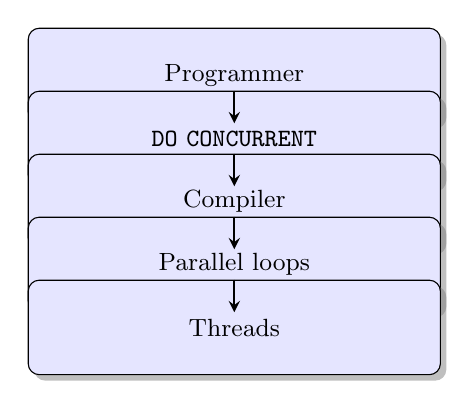
\begin{tikzpicture}[node distance=0.8cm, auto]
			\tikzset{
				block/.style = {rectangle, draw, fill=blue!10, text width=5cm, text centered, 
					minimum height=1.2cm, rounded corners, drop shadow, font=\small},
				arrow/.style = {thick, ->, >=stealth}
			}
			
			\node [block] (programmer) {Programmer};
			\node [block, below of=programmer] (doconcurrent) {\texttt{DO CONCURRENT}};
			\node [block, below of=doconcurrent] (compiler) {Compiler};
			\node [block, below of=compiler] (parallel) {Parallel loops};
			\node [block, below of=parallel] (threads) {Threads};
			
			\draw [arrow] (doconcurrent) -- (programmer);
			\draw [arrow] (compiler) -- (doconcurrent) ;
			\draw [arrow] (parallel) -- (compiler);
			\draw [arrow] (threads) -- (parallel);
		\end{tikzpicture}
		\caption{Parallelization flow with DO CONCURRENT.}
		\label{fig:parallel_flow}
	\end{figure}
	
	The workflow is as follows:
	\begin{enumerate}
		\item The \textbf{programmer} expresses the loop using the standard \texttt{DO CONCURRENT} construct.
		\item The \textbf{compiler} analyzes the loop and determines the optimal parallelization strategy.
		\item The compiler generates \textbf{parallel loops}.
		\item The parallel loops are executed across available \textbf{threads} or processing units.
	\end{enumerate}
	
	
	\section{CMake Build System}
	
	The repository uses CMake as the build system, providing:
	
	\begin{itemize}
		\item Cross-platform support (Linux, Windows).
		\item Support for multiple compilers (Intel ifx, NVIDIA nvfortran).
		\item Automatic detection of compiler capabilities.
		\item Configuration of single/double precision at compile time.
	\end{itemize}
	
	
	\section{Benchmarking Methodology}
	\label{sec:methodology}
	
\begin{table}[h]
	\centering
	\caption{Benchmark platforms used for performance evaluation.}
	\label{tab:benchmark_platform}
	\begin{tabular}{lll}
		\hline
		\textbf{Component} & \textbf{Platform 1} & \textbf{Platform 2} \\
		\hline
		Processor & Intel Core i5 (8th Generation) & AMD Ryzen 9 3900XT \\
		Operating System & Windows 11 & Ubuntu (WSL2) \\
		Compiler & Intel oneAPI ifx 2026 & NVIDIA HPC SDK nvfortran 24.5 \\
		Physical Cores & 4 & 12 \\
		Logical Threads & 8 & 24 (SMT Enabled) \\
		Parallel Model & DO CONCURRENT & DO CONCURRENT \\
		Precision Modes & Single, Double & Single, Double \\
		Grid Sizes & $1000^2$--$4000^2$ & $1000^2$--$4000^2$ \\
		Time steps & $2,000$ & $2,000$ \\
		Benchmark Metrics & Execution Time, MLUPS & Execution Time, MLUPS \\
		\hline
	\end{tabular}
\end{table}

All benchmarks were performed using identical source code, numerical parameters, and compiler-driven parallelization via the standard Fortran \texttt{DO CONCURRENT} construct. Only the compiler, operating system, hardware platform, thread count, and floating-point precision were varied during the performance evaluation.


%\subsection{Validation}

%The solver was validated through a comprehensive regression testing framework. The conservation of total mass was monitored throughout all simulations, confirming the numerical integrity of the implementation.

	\section{Performance Results}
\label{sec:results}
	
Figure~\ref{fig:scaling} shows the strong scaling results for the NVIDIA HPC SDK (nvfortran) on an AMD Ryzen 9 3900XT processor.
		
	\begin{figure}[!tbp]
	   \centering
	  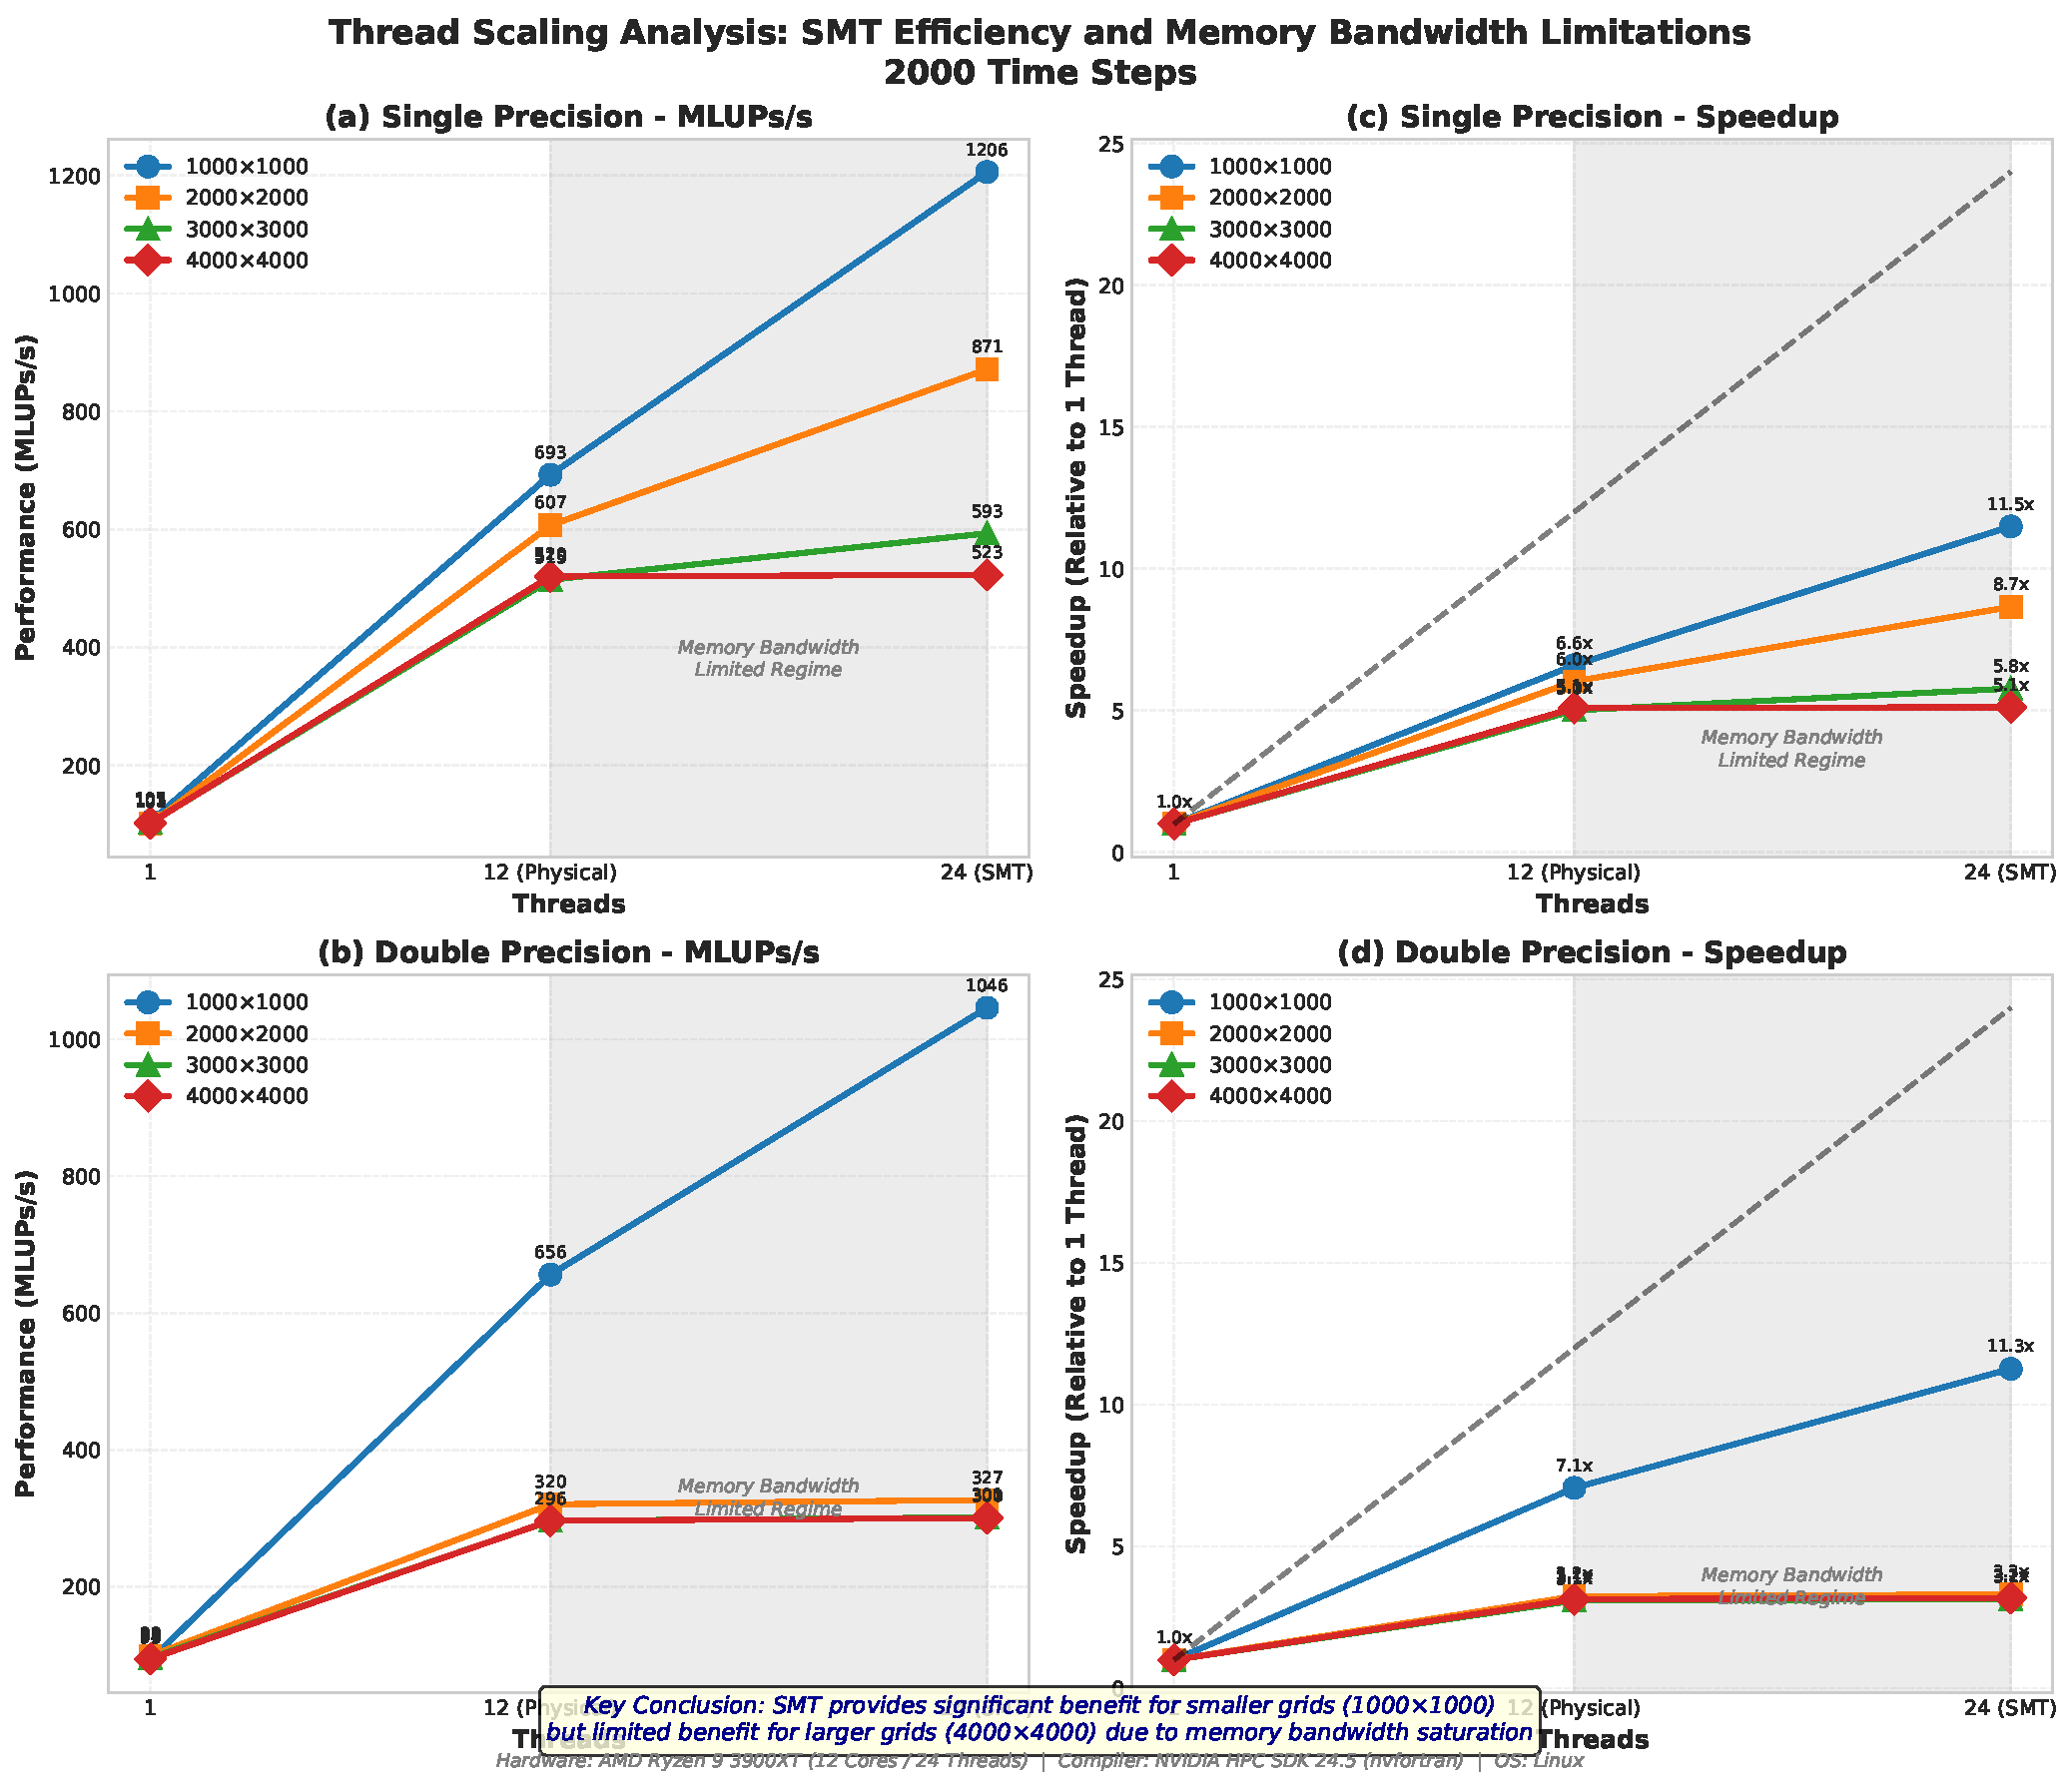
\includegraphics[width=0.9\textwidth]{thread_scaling_combined.pdf}
	 \caption{Strong scaling analysis of the compiler-driven DO CONCURRENT implementation using the NVIDIA HPC SDK (nvfortran) on an AMD Ryzen 9 3900XT processor. The figure compares performance across 1, 12, and 24 threads, highlighting the influence of SMT and memory-bandwidth limitations for a fixed workload of 2000 time steps.}
	 \label{fig:scaling}
	\end{figure}

	
	\begin{figure}[H]
	\centering
	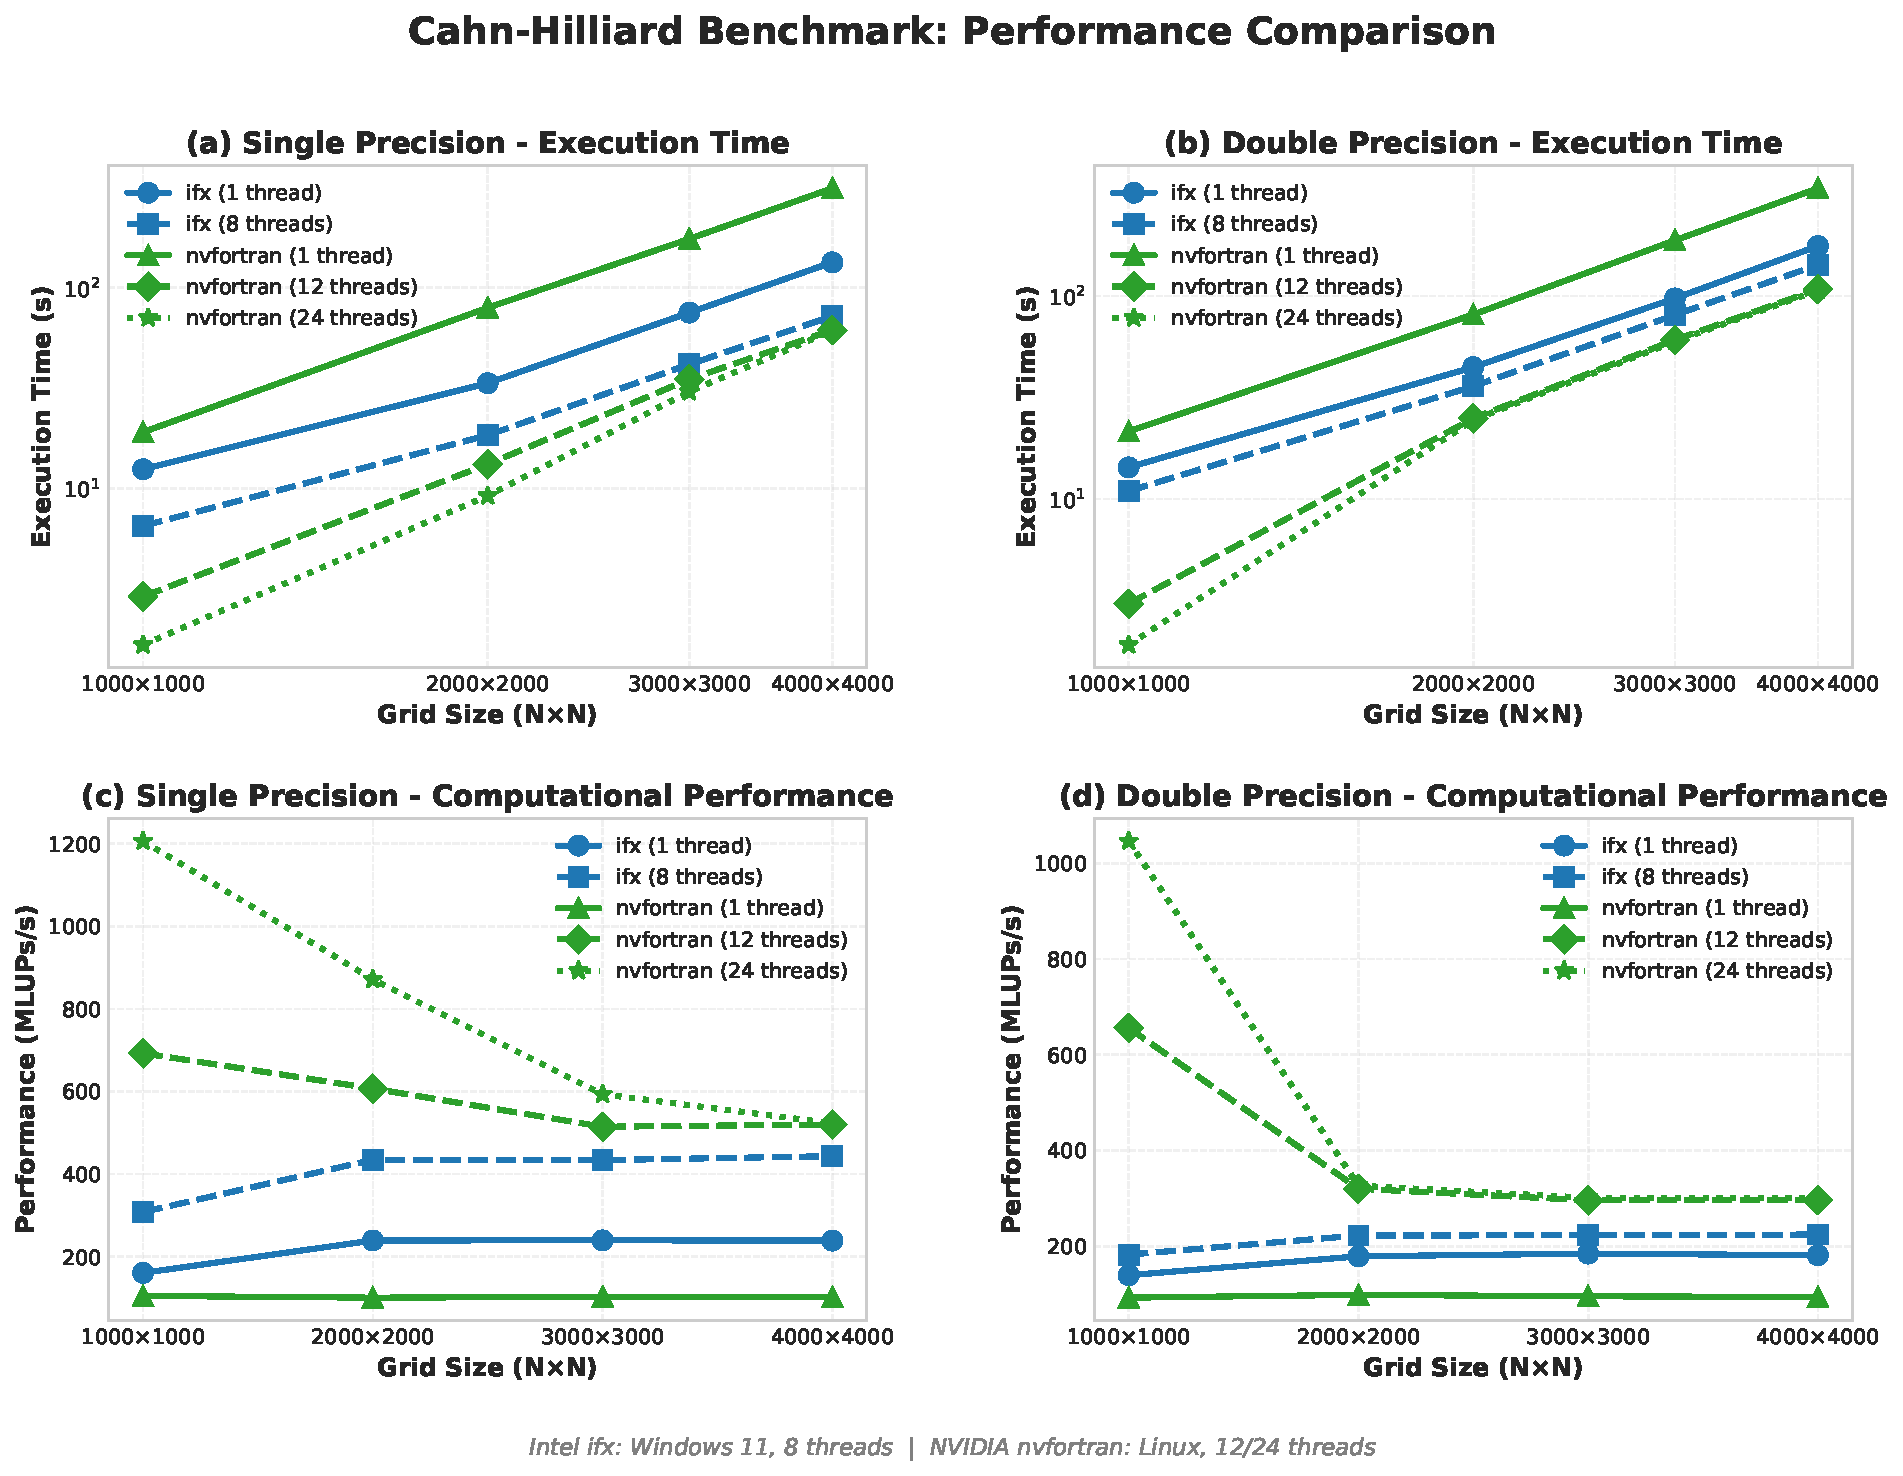
\includegraphics[width=1.0\textwidth]{figure1_performance_comparison.pdf}
	\caption{Execution time and computational performance
		comparison between Intel ifx and NVIDIA nvfortran
		for single- and double-precision implementations.}
	\label{fig:performance_comparison}
	\end{figure}		
			
	\begin{figure}[H]
	    \centering
	    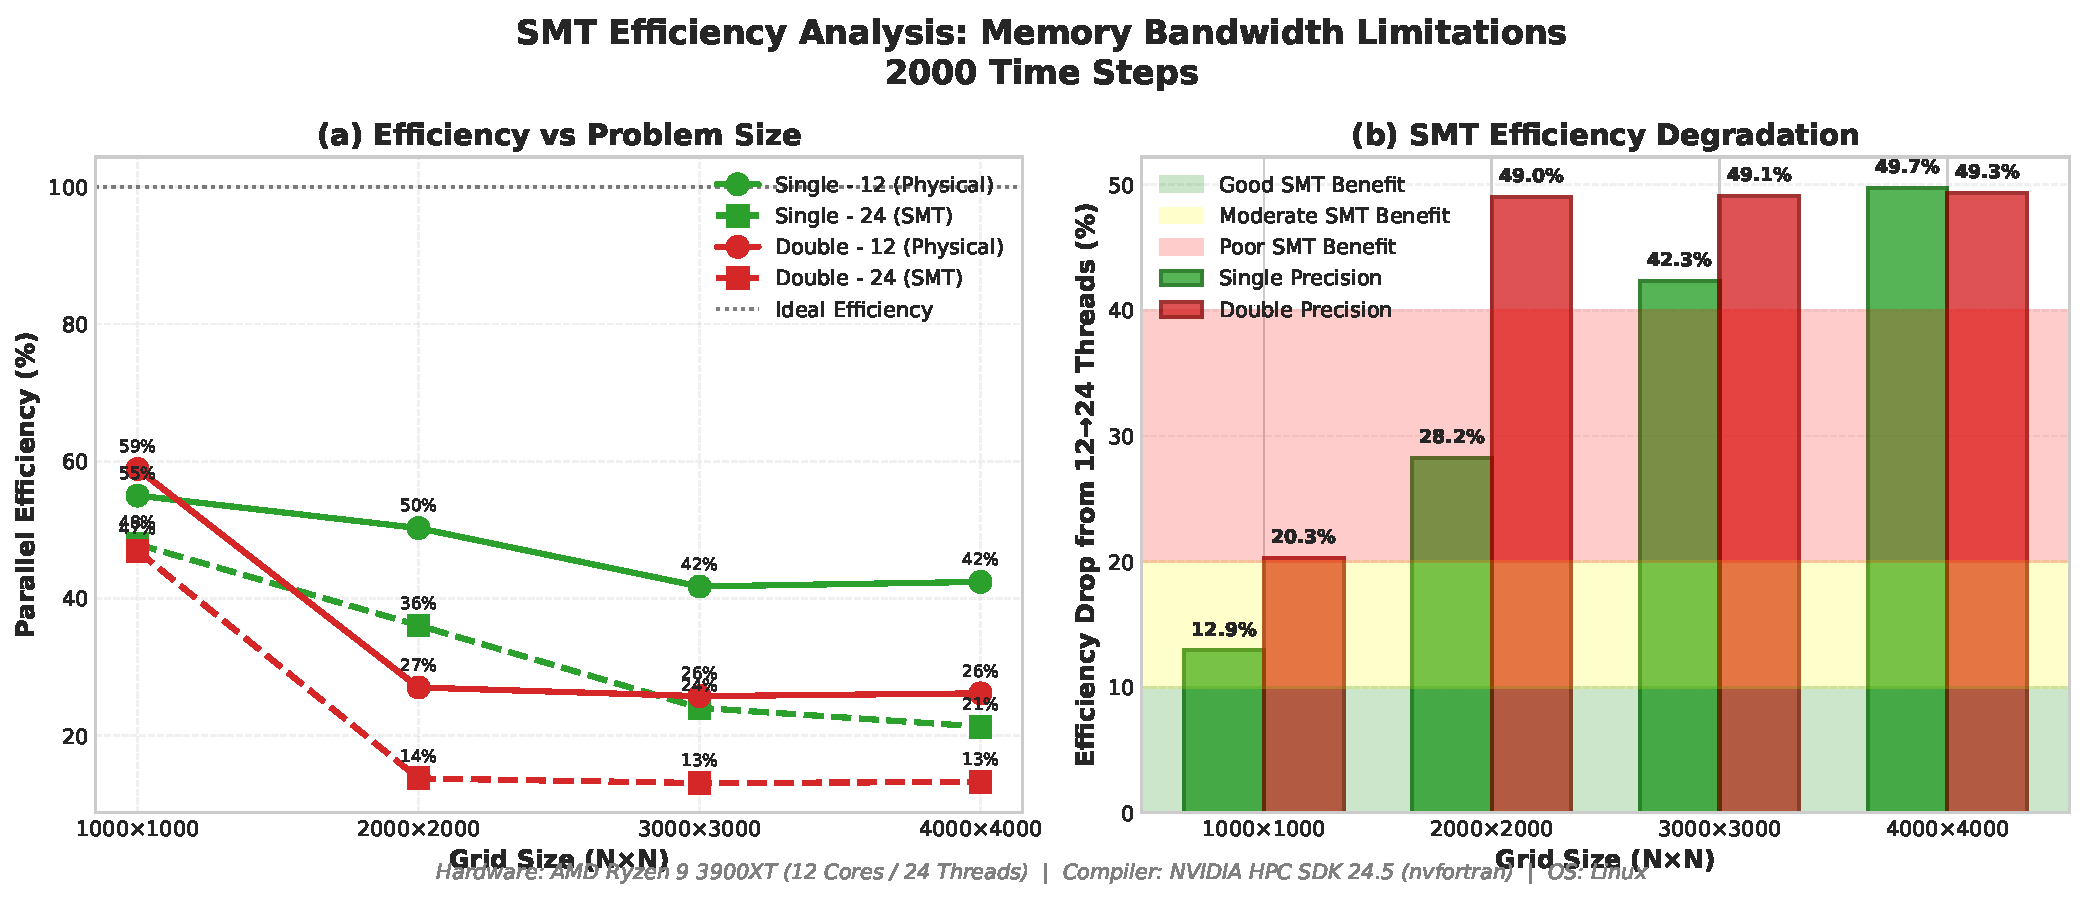
\includegraphics[width=1.0\textwidth]{smt_efficiency_analysis.pdf}
	    \caption{SMT scalability analysis showing the impact of memory-bandwidth limitations on the compiler-driven \texttt{DO CONCURRENT} implementation using NVIDIA nvfortran on an AMD Ryzen 9 3900XT platform.}
	    \label{fig:smt}
	\end{figure}
		
	\section{Discussion}
	
Figure~\ref{fig:scaling} shows the strong scaling performance of the DO CONCURRENT solver over 2000 time steps. The execution time decreases substantially from 1 to 12 threads, demonstrating effective compiler-driven parallelization. However, beyond 12 physical cores, the additional SMT threads provide only marginal improvements due to memory bandwidth limitations. This behavior is typical for memory-bound applications and indicates that the solver's performance is constrained by data movement rather than compute capacity. 

Single precision (Figure~\ref{fig:performance_comparison})  consistently delivers higher throughput than double precision for both compilers. The reduction in performance observed for double precision is expected because each numerical update requires twice the memory traffic. As the grid size increases, the working set exceeds the processor caches, making memory bandwidth the dominant performance constraint. Consequently, the performance gap between single and double precision becomes more apparent for larger computational domains. An important observation is that the achieved MLUPS gradually decreases as the grid size increases for all parallel configurations. Although larger problems provide more computational work, they also place greater pressure on the memory hierarchy, reducing arithmetic intensity and increasing memory-access latency. This behavior is characteristic of memory-bound stencil computations, where overall performance is increasingly limited by memory bandwidth rather than raw computational capability.
	
Figure~\ref{fig:performance_comparison} also shows Intel ifx trailing NVIDIA nvfortran in absolute throughput across both precisions. This gap should not be read as a statement about \texttt{DO CONCURRENT} parallelization itself — optimization reports generated during compilation (-qopt-report=3) confirm that ifx genuinely transforms \texttt{DO CONCURRENT} loops into multithreaded regions, in the same way nvfortran does. Rather, the two platforms in Table 2 differ in more than compiler: Platform 1 has 4 physical cores against Platform 2's 12, and runs natively on Windows 11 rather than native Linux. With three times fewer physical cores available, and with \texttt{DO CONCURRENT} regions launched fresh each time step over 2,000 time steps, Platform 1 has both a lower ceiling on achievable parallelism and proportionally more thread fork/join overhead to amortize per unit of useful work. The comparison in Figure~\ref{fig:performance_comparison} is therefore illustrative of two representative platforms rather than a controlled, single-variable measurement of compiler performance; isolating the compiler as the sole independent variable, by benchmarking ifx on the same AMD Ryzen 9 3900XT platform used for the nvfortran results, is identified as near-term future work.	
	
	
 For Figure~\ref{fig:smt} with the smallest problem size ($1000 \times 1000$), enabling SMT provides a noticeable improvement in computational efficiency. This indicates that the processor is able to utilize otherwise idle execution resources when the workload is relatively small, allowing the additional logical threads to contribute useful work. As the problem size increases, however, the benefit of SMT decreases substantially. For grid sizes of $2000 \times 2000$ and larger, the improvement obtained by increasing the thread count from 12 to 24 becomes progressively smaller, and the efficiency gap between physical-core execution and SMT execution widens. This trend is observed consistently for both single- and double-precision simulations.

	\section{Conclusion}
	\label{sec:conclusion}
	
	This report has presented the design and implementation of a modern Fortran Cahn–Hilliard solver using the Fortran 2008 \texttt{DO CONCURRENT} construct. The primary objective — demonstrating portable, compiler-driven parallelism without vendor-specific directives — was achieved: a single, unmodified source tree was compiled and parallelized by two independent compiler vendors (Intel oneAPI and NVIDIA HPC SDK) using only standard Fortran.
	
	key findings:
	
	\begin{itemize}
	\item \texttt{DO CONCURRENT} provides a portable, standard-compliant path to loop-level parallelism in Fortran, eliminating the need for vendor-specific directives such as OpenMP or OpenACC. This was confirmed directly, not just inferred from timing: compiler optimization reports (-qopt-report) show \texttt{DO CONCURRENT} loops being outlined into genuine multithreaded regions on both compilers.
	
	

	\item Both compilers deliver substantial multi-core speedup from physical cores alone — up to 7.1 $\times$ on 12 physical cores (NVIDIA HPC SDK, double precision, Figure {\ref{fig:scaling}} — confirming that \texttt{DO CONCURRENT} is a practical, working parallelization strategy for this class of stencil computation.
	

	\item Scaling is memory-bandwidth-limited beyond the physical core count, not compute-limited. Parallel efficiency on the NVIDIA HPC SDK platform ranges from 59 $\%$ down to 13 to 26 $\%$ at larger grid sizes with SMT enabled (Figure 6), and additional logical (SMT) threads provide only marginal benefit once the working set exceeds cache capacity. This is the expected, textbook signature of a memory-bound stencil code, not a shortcoming of  \texttt{DO CONCURRENT} itself — it reflects the arithmetic intensity of the Cahn–Hilliard update, not the parallelization mechanism.
	
	\item The single-precision-vs-double-precision performance gap widens with grid size (Figure \ref{fig:smt}), consistent with double precision's doubled memory traffic becoming the dominant cost as problems grow beyond cache.
	
	\item The cross-compiler comparison in Figure \ref{fig:smt} was run on two different hardware platforms (Table \ref*{tab:benchmark_platform}) and should be read as an illustrative comparison rather than a controlled one; isolating the compiler as the sole independent variable is identified as near-term future work below.
	
	\end{itemize}
	
	\subsection{Future work}
		\begin{itemize}
	\item Repeat the Intel oneAPI benchmark on the same AMD Ryzen 9 3900XT platform used for the NVIDIA HPC SDK results, isolating compiler choice as the only variable and enabling a directly controlled ifx-vs-nvfortran comparison.
	
	\item Optimize the periodic-boundary indexing in the Laplacian kernel (currently branch-computed per element) using ghost/halo cells, removing the gather-load penalty identified in the Intel vectorization reports and re-evaluating its contribution to overall performance.
	
	\item Extend the test suite to exercise the production `src/` modules directly, including a mass-conservation check ( invariance over time) as a numerical correctness safeguard.
	
	\item Extend the solver to 3D grids.
	
	\item Explore hybrid MPI + \texttt{DO CONCURRENT} parallelization for distributed-memory systems.
	
	\item Pursue native GPU offloading via \texttt{DO CONCURRENT}, building on the CPU-parallel results presented here.
	
	\end{itemize}
		
\end{document}